\documentclass[fleqn]{jbook}
\usepackage{physpub}

\begin{document}

\begin{question}{専攻 問題5}{}

固体結晶内の電子について次の問に答えよ。
\begin{subquestions}
\SubQuestion
  結晶内で周期的に変化するポテンシャル場$U(\vec{r})$の中を運動する
  電子に対するシュレーディンガー方程式
%
  \[ H\Psi=\left(-\frac{\hbar^2}{2m}\vec{\nabla}^2+U(\vec{r})\right)
     \Psi=E\Psi,\hspace{1cm} U(\vec{r}+\vec{R})=U(\vec{r}) \]
%
  の固有関数$\Psi(\vec{r})$は、$\vec{k}$を波数ベクトルとするとき
%
  \begin{equation}
    \Psi(\vec{r}+\vec{R})=e^{i\vec{k}\vec{R}}\Psi(\vec{r}) \eqname{1}
  \end{equation}
%
  という性質(ブロッホの定理)を持つことを示せ。ただし、$m$は電子質量で、
  $\vec{R}$は格子ベクトルで基本ベクトル$\vec{a}_i$と整数$n_i(i=1,2,3)$
  を用いて $\vec{R}=n_1\vec{a}_1+n_2\vec{a}_2+n_3\vec{a}_3$と表される。


\SubQuestion
  一次元空間において異なる二種類の原子AとBがそれぞれ
  $x=na,na+b\quad(n=0,\pm1,\pm2,\pm3,\cdots,0<b<a)$ の位置に交互に
  並んだ二原子結晶において、強く原子に束縛された電子のエネルギー
  バンドを求めることを考える。A原子とB原子が孤立した時に電子が受ける
  ポテンシャルをそれぞれ$U_A(x),U_B(x)$、その時の原子軌道関数を
  $\phi_A(x),\phi_B(x)$(共に実数とする)、固有エネルギーを$E_A,E_B$
  とし、結晶のハミルトニアンを
%
  \[ H=-\frac{\hbar^2}{2m}\Deriver{^2}{x^2}+U(x) \hspace{15mm}%
     U(x)=\sum_nU_A(x-na)+\sum_nU_B(x-na-b) \]
%
  とする。原子間の相互作用としては隣り合う原子間のポテンシャルを介した
  相互作用のみを考え、隣り合う原子軌道関数同士の単なる重なり積分
  (非直交性)は無視するものとする。

  \begin{subsubquestions}
  \SubSubQuestion
    各原子の波動関数を用いて近似した線形結合の式
%
    \[ \Psi_A(x) = \frac{1}{\sqrt{N}}\sum_ne^{ikna}\phi_A(x-na)%
       \hspace{15mm}%
       \Psi_B(x) = \frac{1}{\sqrt{N}}\sum_ne^{ikna}\phi_B(x-na-b) \]
%
    はブロッホの条件式\eqhref{1}を満足することを示せ。ただし、$N$は
    結晶全体に含まれる単位格子の数である。

  \SubSubQuestion
    ハミルトニアン$H$の$\Psi_A,\Psi_B$に対する行列要素
%
    \[ H_{AA},H_{BB},H_{AB},H_{BA} \]
%
    を求めよ。ただし、隣り合う軌道関数同士の重なり積分を無視するときは
%
    \begin{eqnarray*}
      \gamma&%
      \equiv& \Uint{\d{x}} \phi_A(x)U_A(x)\phi_B(x-b)
       =      \Uint{\d{x}} \phi_A(x)U_B(x-b)\phi_B(x-b) \\
      &=&     \frac{1}{2}\Uint{\d{x}}\phi_A(x)\{U_A(x)+U_B(x-b)\}\phi_B(x-b)\\
      \gamma'&%
      \equiv& \Uint{\d{x}} \phi_A(x)U_A(x)\phi_B(x+a-b)
       =      \Uint{\d{x}} \phi_A(x)U_B(x+a-b)\phi_B(x+a-b) \\
      &=&     \frac{1}{2}\Uint{\d{x}}\phi_A(x)\{U_A(x)+U_B(x+a-b)\}\phi_B(x+a-b) 
    \end{eqnarray*}
%
    としてよい。

  \SubSubQuestion
    $E_A,E_B,\gamma,\gamma'$を用いて固有エネルギー$E(k)$を求めよ。
    エネルギーバンドの図を横軸を波数$k$、縦軸をエネルギー$E(k)$
    として描け。

  \SubSubQuestion
    エネルギーバンドのギャップと各バンドの幅を求めよ。

  \SubSubQuestion
    第一ブリルアン域($-\pi/a\leq k<\pi/a$)の中に含まれる全状態数は
    どれだけか、また、A,B原子が各一個ずつ電子を持つ時、電子はバンド
    内にどのように分布するか。

  \end{subsubquestions}
\end{subquestions}
\end{question}
\begin{answer}{専攻 問題5}{}

\begin{subanswers}
\SubAnswer
  並進演算子$T_{\vec{R}}$ を次のように定義する。
%
  \[ T_{\vec{R}} f(\vec{r}) = f(\vec{r}+\vec{R}) \]
%
  ハミルトニアン${\cal H}$ は周期的であるから
%
  \[ T_{\vec{R}}{\cal H}(\vec{r}) \psi(\vec{r})%
     = {\cal H}(\vec{r}+\vec{R})\psi(\vec{r}+\vec{R})%
     = {\cal H}(\vec{r})\psi(\vec{r}+\vec{R})%
     = {\cal H}(\vec{r})T_{\vec{R}}\psi(\vec{r}) \]
%
  よって ${\cal{H}}$ と $T_{\vec{R}}$ は交換可能。
  よって、${\cal{H}}$と $T_{\vec{R}}$は同時対角化可能 
  なので ${\cal{H}}$ の固有波動関数 $\psi$ について
%
  \[ T_{\vec{R}}\psi=C(\vec{R})\psi \]
%
  となる固有値 $C(\vec{R})$ が存在する。
  (但し、$T_{\vec{R}} {\cal{H}}(\hat{x})T^{\dag}_{\vec{R}} = {\cal{H}}(\hat{x}+\vec{R})$に注意。) \\
%  並進演算子はその性質から
%
%  \[  T_{\vec{R}_1} T_{\vec{R}_2}%
%    = T_{\vec{R}_2} T_{\vec{R}_1}%
%    = T_{\vec{R}_1+\vec{R}_2} \]
%
%  であるので、
%
%  \[  T_{\vec{R}_1} T_{\vec{R}_2} \psi%
%    = T_{\vec{R}_1+\vec{R}_2} \psi%
%    = C(\vec{R}_1+\vec{R}_2) \psi \]
%  \[  T_{\vec{R}_1} T_{\vec{R}_2} \psi%
%    = T_{\vec{R}_1} C(\vec{R}_2) \psi%
%    = C(\vec{R}_1) C(\vec{R}_2) \psi \]
%  \[ \Yueni C(\vec{R}_1+\vec{R}_2) = C(\vec{R}_1) C(\vec{R}_2) \]
%
%  が導かれる。このような積の性質をもつ関数は指数関数しかない。
%  並進操作を無限回繰り返しても波動関数は有限であるので $|C|=1$で
%  なければならないので、$C(\vec{R})$の表式は
%
%  \[ C(\vec{R}) = e^{i\vec{k}\cdot\vec{R}} \]
%
  表面の影響を無視するため、ボルン・フォン・カルマンの周期的境界条件:$(N_1,N_2,N_3)$だけ並進して元に戻る、つまり、
 \[ \psi(\vec{x}+N_j\vec{a_j})=C(\vec{a_j})^{N_j}\psi(\vec{x})=\psi(\vec{x})
      \quad (j=1,2,3) \]
とする。よって、
 \[ C(\vec{a_j})=e^{i\frac{2\pi}{N_j}l_j} \quad (l_j=0,1,2,\cdots N_j-1) \]
 \[ \Yueni \psi(\vec{x}+\vec{R})=C(n_1\vec{a_1})C(n_2\vec{a_2})C(n_3\vec{a_3})
                               \psi(\vec{x})
           =\exp(i\sum_{j} \frac{2\pi}{N_j}l_j n_j )\psi(\vec{x}) 
           =\exp(i\vec{k}\cdot \vec{R}) \psi(\vec{x}) \]
  となる。ここで $\vec{k}=(\frac{2\pi}{N_1 a}l_1,\frac{2\pi}{N_2 a}l_2,\frac{2\pi}{N_3 a}l_3)$(結晶波数)であるが、逆格子ベクトル
  $\vec{G}$ の整数倍の自由度をもつ。
  \[\Naze   e^{i(\vec{k}+n\vec{G})\cdot\vec{R}}%
    = e^{i\vec{k}\cdot\vec{R}}e^{in\vec{G}\cdot\vec{R}}%
    = e^{i\vec{k}\cdot\vec{R}} \]
%
  だからである。また、
\[ \psi(\vec{x}+\vec{a_j})=(1+a_j\Deriver{}{x_j}+\frac{1}{2!}a_j^2 \Deriver{^2}{x_j^2}+\cdots )\psi(\vec{x})=e^{a_j \Deriver{}{x_j}}\psi(\vec{x})=e^{\frac{i}{\hbar}\vec{a_j}\cdot \vec{p}}\psi(\vec{x}) \]
となり、$\vec{k}$は波数ベクトルに他ならない。よって
%
  \[ T_{\vec{R}} \psi(\vec{r}) = \psi(\vec{r}+\vec{R})%
                               = e^{i\vec{k}\cdot\vec{R}}\psi(\vec{r}) \]
%
  が示された。


\SubAnswer
  \begin{subsubanswers}
  \SubSubAnswer
%    格子一つ分だけ並進する場合のブロッホの定理を満たすことを
%    示せば十分である。すなわち、
%
%    \[ \psi(x+a) = e^{ika} \psi(x) \]
%
    $R=ma(0\leq m<N)$だけ並進した場合を考える。
%    与えられた $\Psi_A(x)$ がこれを満たすかを検証する。
%
\begin{eqnarray*}
     \Psi_A(x+ma)%
   &= & e^{ikma}\frac{1}{\sqrt{N}}\sum_{n=1}^{N}e^{ik(n-m)a}\phi_A(x-(n-m)a)%
      =e^{ikma}\frac{1}{\sqrt{N}}\sum_{n=1-m}^{N-m}e^{ikna}\phi_A(x-na)\\
   &= & e^{ikma}\frac{1}{\sqrt{N}}(\sum_{n=1}^{N-m}+\sum_{n=1-m}^0) e^{ikna}\phi_A(x-na)  
\end{eqnarray*}
%
%    $n=0$の原子軌道から寄与は十分小さいと考えられるので、$\sum_{n=0}^{N-1}$を
%    $\sum_{n=1}^{N}$と同一視することができる。よって、
%     ただし、最後の等号には、周期的境界条件$\phi(x+Na)=\phi(x)$を
%     用いた。よって、
%
   周期的境界条件から、$\phi(x+Na)=\phi(x)$なので、
\begin{eqnarray*}
 \Psi_A(x+ma)%
    &=& e^{ikma}\frac{1}{\sqrt{N}}\sum_{n=1}^{N-m}e^{ikna}\phi_A(x-na)
          +\sum_{n=1-m}^0 e^{ik(N+n)a}\phi_A(x-(N+n)a) \\
    &=& e^{ikma}\frac{1}{\sqrt{N}}\sum_{n=1}^N e^{ikna}\phi_A(x-na) 
     =e^{ikma} \Psi_A(x)   
\end{eqnarray*} 
%    \[ \Psi_A(x+a) =  e^{ika} \Psi(x) \]
%
    となり、ブロッホの定理が満たされていることが示された。\\
%
    $\Psi_B(x)$についても同様に示される。


  \SubSubAnswer
    行列要素 $H_{\rm AA}$ は
%
    \[ H_{AA}%
       = \Uint{\d{x}} \Psi_A^{\ast}(x) {\cal H} \Psi_A(x) \]
%
    であり、これに与えられた表式を代入して計算する。\\
%
    その計算において、与えられた仮定より原子軌道の重なり積分は
    無視できる。すなわち
%
    \[ \Uint{\d{x}} \phi_A^{\ast}(x-na) \Deriver{^2}{x^2} \phi_A(x-ma) = 0%
       \hspace{32mm} {\rm for}\quad n \neq m \]
%
    またポテンシャルを介した相互作用は隣接AB原子間のみに働くので
    異なるA原子の軌道同士には働かない。すなわち
%
    \[ \Uint{\d{x}} \phi_A^{\ast}(x-na) U_A(x-la) \phi_A(x-ma) = 0%
       \hspace{21mm} {\rm for}\quad n \neq m \]
    \[ \Uint{\d{x}} \phi_A^{\ast}(x-na) U_B(x-la-b) \phi_A(x-ma) = 0%
       \hspace{15mm} {\rm for}\quad ^{\forall} n,m \]
%
    以上を踏まえると $H_{\rm AA}$ は
%
    \begin{eqnarray*}
      H_{\rm AA} &=& \frac{1}{N} \sum_{n} \Uint{\d{x}}%
                 \phi_A^{\ast}(x-na)\Bigl[%
                   -\frac{\hbar^2}{2m}\Deriver{^2}{x^2} + U_A(x-na)
                 \Bigr]\phi_A(x-na) \\
             &=& \Uint{\d{x}} \phi_A^{\ast}(x)\Bigl[%
                   -\frac{\hbar^2}{2m}\Deriver{^2}{x^2} + U_A(x)
                 \Bigr]\phi_A(x)
    \end{eqnarray*}
%
    この表式は $\phi_A(x)$ が局在化した場合の固有エネルギー $E_A$ に
    他ならない。 $H_{\rm BB}$についてもまったく同様である、
%
    \[ H_{\rm AA} = E_A \hspace{10mm} H_{\rm BB} = E_B \]
%
    次に $H_{\rm AB}$ は、これもまた原子軌道の重なり積分は
    無視できるので
%
    \[ \Uint{\d{x}} \phi_A^{\ast}(x-na) \Deriver{^2}{x^2} \phi_B(x-ma-b) = 0%
       \hspace{27mm} {\rm for}\quad ^{\forall} n,m \]
%
    ポテンシャルの相互作用は隣接するAB原子間の軌道では
%
    \[ \Uint{\d{x}} \phi_A^{\ast}(x-na)%
         \{U_A(x-na)+U_B(x-na-b)\}
       \phi_B(x-na-b)\d{x} = 2\gamma  \]
%
    隣接するBA原子間の軌道では
%
    \[ \Uint{\d{x}} \phi_A^{\ast}(x-na)%
         \{U_A(x-na)+U_B(x-na+a-b)\}
       \phi_B(x-na+a-b) = 2\gamma' \]
%
    となる。以上を踏まえると $H_{\rm AB}$ は
%
    \begin{eqnarray*}
      H_{\rm AB} &=& \frac{1}{N}\! \sum_{n}\!\! \Uint{\d{x}}%
                 e^{-ikan}\phi_A^{\ast}(x\!-\!na)\Bigl[%
                   U_A(x\!-\!na)+U_B(x\!-\!na\!-\!b)
                 \Bigr]e^{+ikan}\phi_B(x\!-\!na\!-\!b) \\
                 &+& \frac{1}{N}\! \sum_{n}\!\! \Uint{\d{x}}%
                 e^{-ikan}\phi_A^{\ast}(x\!\!-\!\!na)\Bigl[%
                   U_A(x\!-\!na)+U_B(x\!-\!na\!+\!a\!-\!b)
                 \Bigr]e^{+ika(n-1)}\phi_B(x\!-\!na\!+\!a\!-\!b) \\
             &=& \frac{1}{N} \sum_{n} (2\gamma+2\gamma' e^{-ika})\\
             &=& 2\gamma+2\gamma'e^{-ika}%
    \end{eqnarray*}
%
    と求まる。最後に  $H_{BA}$ は
%
    \[ H_{\rm BA} = H_{\rm AB}^{\ast} = 2\gamma+2\gamma'e^{+ika} \]
%
    である。
 
  \SubSubAnswer
    ハミルトニアンの行列表現は
%
    \[ {\cal{H}} =\begin{pmatrix}
                    E_A & 2\gamma + 2\gamma^{\prime} e^{-ika} \\ 
                    2\gamma + 2\gamma^{\prime} e^{ika} & E_B \cr \end{pmatrix} \] 
%
    である。この固有値 $E^{\pm}$を求めと。
%
    \[ E^{\pm}=\frac{1}{2} \left(%
           E_A+E_B \pm \sqrt{(E_A-E_B)^2+16(\gamma^2+2\gamma\gamma^{\prime} \cos ka +{\gamma^{\prime}}^2)}%
         \right) \]
%
    と求まる。この2種の固有エネルギーの$k$依存性は下図の通りである。
%
    \begin{center}
      \mbox{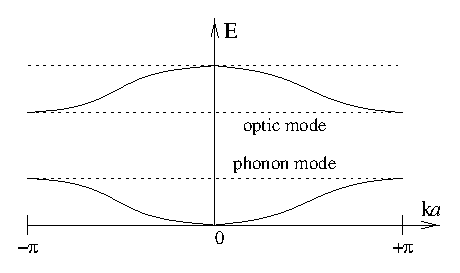
\includegraphics[clip]{1993phy5-1.eps}}
    \end{center}
%

  \SubSubAnswer
    バンドギャップは光学モードと音響モードとの間のエネルギー差の
    最小値である。
%
    \[ E_{\rm band gap} = {\rm min}(E^{+} - E^{-}) %
          = \sqrt{(E_A-E_B)^2+16(\gamma-\gamma^{\prime})^2} \]
%
    バンドの幅は光学モードと音響モードと共に同じで
%
    \[ E_{\rm band width}%
        = \sqrt{(E_A-E_B)^2+16(\gamma+\gamma^{\prime})^2}%
         -\sqrt{(E_A-E_B)^2+16(\gamma-\gamma^{\prime})^2} \]


  \SubSubAnswer
    第1Brillouin zone には$2N$ の状態がある。
    A,B 原子が1つずつ電子をもっていると$2N$ の電子があるから
    第1 Brillouin zone の音響モードがうめつくされる。

  \end{subsubanswers}
\end{subanswers}
\end{answer}


\end{document}
